% Metódy inžinierskej práce
\documentclass[10pt,twoside,a4paper]{article}

%\usepackage[slovak]{babel}
%\usepackage[T1]{fontenc}
%\usepackage[IL2]{fontenc} % lepšia sadzba písmena Ľ než v T1
\usepackage[utf8]{inputenc}
\usepackage{graphicx}
\usepackage{url} % príkaz \url na formátovanie URL
\usepackage{hyperref} % odkazy v texte budú aktívne (pri niektorých triedach dokumentov spôsobuje posun textu)
\usepackage{lipsum}
\usepackage{csquotes}

\usepackage{cite}

\pagestyle{headings}

\title{Getting information to the user optimally\thanks{Semestrálny projekt v predmete Metódy inžinierskej práce, ak. rok 2023/24, vedenie: Ing. Ivan Kapustík}}

\author{Samuel Tvrdoň\\[2pt]
	{\small Slovenská technická univerzita v Bratislave}\\
	{\small Fakulta informatiky a informačných technológií}\\
	{\small \texttt{xtvrdon@stuba.sk}}
	}

% TODO:
\date{\small 5. november 2023} % upravte

\begin{document}

\maketitle

\begin{abstract}
Getting the user, the information they seek as quickly and efficiently as possible is key when talking about searching in today’s world. his article chooses to focus on the ways this is achieved behind the scenes. Comparing different indexing techniques and other optimizations modern database engines employ to provide optimal storage and retrieval efficiency. The article also looks at methods of making retrieval faster by utilizing caching in a way that increases the performance of storage access. Furthermore, querying the database for data the user wants quickly, would not be possible without proper tokenization of the data in the database. The methods for tokenization are also mentioned in the last section of the article.
\end{abstract}

\section{Introduction}
With the ever growing expectations from the side of the users, database technologies are always evolving.\cite{Database-indexing:-yesterday-and-today} Fighting for the users attention means bringing up the requested information as quickly as possible. Since the inception of the internet there have been many advancements in the field of information storage and retrieval that are now common place in almost every large application. There are of course benefits and pitfalls each of the performance improvement techniques brings. The first part of article aims to describe indexing its strengths and also multiple ways to create an index for a database table. Moreover, even more performance can be gained by predicting, which data will be used the most and storing it in a faster storage with caching. Additionally the article goes over turning natural language searches into efficient database queries. In this section the article explains how tokenization is used to achieve natural search feeling from the users perspective, while maintaining optimal speeds.

\section{Indexing}
Indexing is used to make querying data faster and more efficient. Since the data can be any size,
and stored in any order, going over every record is unfeasible. With the amount of requests users around the globe make, the equipment costs grow rapidly. To solve this issue, indexing has been introduced as a method to help avoid the need of traversing all of the data on each request. From a report by one of the largest search engines in the world Google\cite{Google}:
\begin{displayquote}
The Google Search index contains hundreds of billions of webpages and is well over 100,000,000 gigabytes in size. It’s like the index in the back of a book — with an entry for every word seen on every webpage we index. When we index a webpage, we add it to the entries for all of the words it contains.
\end{displayquote}

Indices can be created for each of the parameters that needs to be sorted separately. This reduces storage requirements, drastically. Instead of choosing between searching the table each time and having multiple copies of the table ordered by different columns, a third option is now possible. Storing only references to the real table along with the ordered indices. This arrangement is shown in the first figure.\ref{fig:index-city}

Another benefit of indices is their reference to the table is only one directional. In other words the table does not care about how many different indices exist, which provides for easy manipulation and flexibility when iterating over database design.

However, indexing isn't one size fits all, there are many options, which cut different corners and make needed optimizations for even faster querying.
\cite{10.1007/978-3-319-93803-5_1}

\begin{figure}
    \centering
    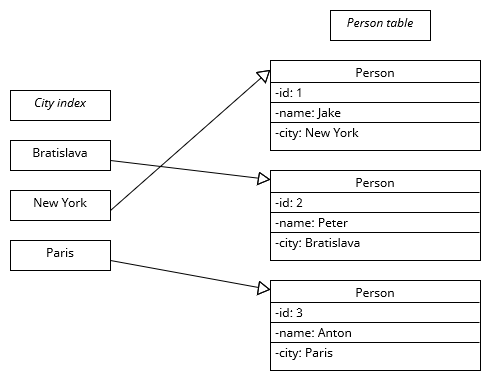
\includegraphics[width=1\linewidth]{Indexing.png}
    \caption{Example of indexing by city name}
    \label{fig:index-city}
\end{figure}

\subsection{Creating an effective key}
As mentioned in the above paragraph, the performance improvement indexing provides is dependent on the data stored in the database.
Take the example in Figure 1 again\ref{fig:index-city}. The id column is unique for each person, making it a prime candidate for an index key. However, the index must also be a value users look up the data by, making the name or the city column more fitting. The problem is the name and city are not required to be unique for each person. This fact reduces the performance increase they would provide. These facts make indexing a balancing act based on the user's needs and the stored data. The uniqueness of values in a database column is measured as cardinality. And in the recent years there have been attempts to choose optimal columns for indexing using the help of artificial intelligence.\cite{li2023stone}

\section{Caching}
In every system each record is accessed with varying frequency. This fact is leveraged by caching. Caching layer makes for even faster retrieval of the most used records. The most queried records are stored in a temporary memory with faster read speeds than the main larger memory. This helps reduce time as well as the stress on the main storage. \cite{10.1145/3009837.3009891}

\subsection{Accessing cache}
The cache layer is a system detached from the main database. This fact allows for different implementations not tied to the underlying database used. This sections aims to look into the most popular arrangements and their pros and cons.\cite{AWS}\cite{Prisma}

\subsubsection{Cache-aside}
\label{sec:cache-aside}
In this arrangement, users first request from the cache. If there is a cache hit, the cache has the requested data and it is returned. If there is a cache miss, the database needs to be queried and the data subsequently returned and stored in the cache for next request. The benefits are in its simplicity and usefulness in general use cases mainly with high read intensity. 
% read-heavy workloads Fit for search engines. 
Cons arise when writing is involved as the speed benefits are lost when any write has to be synced between cache and the database.

\begin{figure}[h]
    \centering
    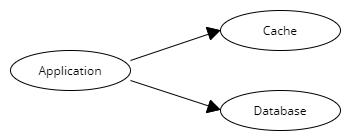
\includegraphics[width=0.5\linewidth]{Cache-aside.png}
    \caption{Cache aside}
    \label{fig:cache-aside}
\end{figure}

\subsubsection{Cache-through}
Very similiar to Cache-aside \ref{sec:cache-aside} The main difference is in which party is responsible for populating the cache. While in Cache-aside the cache is written to by the application. In Read-through arrangement the cache is hidden behind the database management system. Every request goes through the cache, which then proceeds to call the database. Write-through solves the issue of syncing write changes with the cache. In this arrangement all writes as well as reads go through the cache, which, then calls the database. This setup hides the slow main storage away from the users and lets him only talk with the fast cache.

\begin{figure}[h]
    \centering
    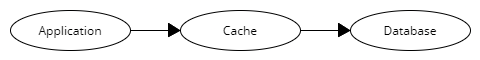
\includegraphics[width=1\linewidth]{Cache-through.png}
    \caption{Cache through}
    \label{fig:cache-through}
\end{figure}

\subsubsection{Cache-back}
In this setup each request goes through the cache, utilizing all the speed benefits the faster storage offers. However, the data isn't immediately passed to the main database, instead the cache passes the data in set intervals, while it is free from load.

\begin{figure}[h]
    \centering
    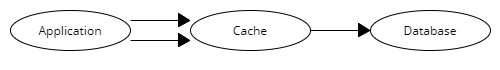
\includegraphics[width=1\linewidth]{Cache-back.png}
    \caption{Cache back}
    \label{fig:cache-back}
\end{figure}

\subsection{Invalidating cache}
Since the cache is way smaller than the main memory. There comes a point when the stored data needs to be cycled. Various algorithms are employed to maximize cache hits and minimize cache misses. Cache invalidation is a technique virtually every modern database system uses. \cite{Redis} This section goes over the most common ones, from the simplest to implement to the more complicated ones. \cite{755618}

\subsubsection{Random replacement}
Random replacement is the simplest form of cache invalidation and is therefore preferred for the simplest of applications. The main benefit comes from the randomness of this approach. There is no need to perform any additional book keeping, like the frequency of access to decide which record to replace. Each piece of cached data is assumed to be just as likely to be accessed in the future so, which one gets removed does not matter.

\subsubsection{First in first out}
The first in first out approach tries to reason about, which data the user might need next. The heuristic reasons that a user is more likely to access data he accessed recently. This algorithm brings in some logic to, which data is replaced, but still keeps it to a minimum, while providing better results.

\subsubsection{Least recently used}
\label{sec:lru}
This strategy chooses to replace items based on the recency of their last access. At its core it is very similar to the First in first out approach, however there is extra logic included. If a piece of data was cached last it can move up the queue when accessed to improve efficiency.

\subsubsection{Least frequently used}
When invalidating entries with the least frequently used heuristic, the data that is accessed the least is assumed to be least likely used in the future as well. Invalidating based on the access frequency means keeping around data that is accessed lots of times. This method provides a benefit over LRU \ref{sec:lru} in access patterns that would invalidate elements accessed in batches.\cite{chand2019comparative}\cite{comparison-cache-replacement}.

% TODO: weaknesses from: https://www.researchgate.net/publication/325014338_A_Comparison_of_Cache_Replacement_Algorithms_for_Video_Services

\section{Tokenization}
% TODO: Tie in with the other sections
Tokenization is what ties information retrieval together. It bridges the gap between natural language and databases. 
Natural language contains many filler words and padding not relevant to the information being searched. To efficiently convert text to a database query it needs to be tokenized. During tokenization the critical parts of each sentence are filtered and used as "tokens". \cite{Effective-Tokenization} %TODO: stemming %TODO stemming diagram 

\section{Conclusion}
In the world of databases there are methods, which if used correctly result in huge performance increases with little added cost. All of the mentioned methods used together make up large part of today's internet infrastructure. Without these optimizations the internet would not be where it is today. These methods may also help create even better optimizations in the future and move data processing to the next level. %TODO:

%\section*{TODO: References}
%\href{https://www.researchgate.net/publication/274837474_An_Effective_Tokenization_Algorithm_for_Information_Retrieval_Systems}{An Effective Tokenization Algorithm for Information Retrieval Systems}\\
%\href{https://dl.acm.org/doi/pdf/10.1145/356643.356645}{HASH TABLE M E T H O D S}\\
%\href{https://ieeexplore.ieee.org/abstract/document/755618?casa_token=1dPMFNh1uOMAAAAA:EhTd5TzTa1RHsWQThUec5nDGgAe82xXTYaG32s8GsTNty9qoUoSPlu0Rzh-it8kQ-qtl19_LX-0KjA}{Caching on the World Wide Web}\\
%\href{https://link.springer.com/chapter/10.1007/978-981-15-6198-6_18}{Study of Various Methods for Tokenization}\\
%\href{https://ieeexplore.ieee.org/abstract/document/1540920?casa_token=hzg5FRuCiVQAAAAA:MDNu1j1gc-DR7xTkOo22jTVIlq55BcYoatyx97bKzY3HdvAw_7-4sRhCNF-iXQcbZQTw2Bb3u0YQxg}{Indexing relational database content offline for efficient keyword-based search}
%\href{https://books.google.sk/books?hl=en&lr=&id=yQgfCgAAQBAJ&oi=fnd&pg=PP1&dq=relational+database&ots=qPKwl0TFYt&sig=6jOwNojMeS_JzJYt9NTVB7_gJwk&redir_esc=y#v=onepage&q=relational%20database&f=false}{Relational Database Design and Implementation}


%\acknowledgement{Ak niekomu chcete poďakovať\ldots}

% týmto sa generuje zoznam literatúry z obsahu súboru literatura.bib podľa toho, na čo sa v článku odkazujete
\bibliography{literatura}
\bibliographystyle{abbrv} % prípadne alpha, abbrv alebo hociktorý iný
\end{document}
